\documentclass{article}
\usepackage{amsmath, sfmath, multicol, tkz-euclide, array, enumerate, tcolorbox, tabularray}
\renewcommand{\familydefault}{\sfdefault}
\setlength{\parindent}{0cm}
\pagestyle{empty}
\usepackage[left=1in, top=0.5in, right=1in, bottom=0.5in]{geometry}
\tikzset{>=stealth}
\tcbset{colback=white}

\newcounter{example}[section]
\newenvironment{example}[1][]{\refstepcounter{example}\par\medskip
   {\color{red}\textbf{Example~\theexample. #1}}}{\medskip}

\begin{document}

\section*{Congruence Transformations}

\begin{tcolorbox}[colframe=orange!70!white, coltitle=black, title=\textbf{Today I Can}]
\begin{enumerate}
    \item Identify congruence transformations.
    \item Prove triangle congruence using isometries.
\end{enumerate}
\end{tcolorbox}
\bigskip 

\begin{example}
The composition $(R_n \circ r_{(90^\circ,P)})(LMNO) = GHJK$ is shown. \newline 

\begin{minipage}{0.55\textwidth}
\begin{enumerate}[(a)]  \setlength{\itemsep}{0.5in}
    \item Which angle pairs have equal measure?
    \item Which sides have equal lengths?
\end{enumerate}
\end{minipage}
\begin{minipage}{0.4\textwidth}
\begin{tikzpicture}[scale=0.7]
    \tkzDefPoints{0/0/J, 0/1/H, 2/1.5/G, 2/0/K}
    \tkzDrawPolygon(J,H,G,K)
    \tkzLabelPoints[left](J,H)
    \tkzLabelPoints[right](G,K)
    \tkzDefPoints{1.5/3/n1, 5/-1/n2}
    \tkzDrawSegment[dashed](n1,n2)
    \tkzLabelLine[below, pos=1](n1,n2){$n$}
    \tkzDefPoints{4.25/1/P}
    \tkzDrawPoint(P)
    \tkzLabelPoints[below](P)
    \tkzDefPointsBy[reflection=over n1--n2](J,H,G,K){Jp,Hp,Gp,Kp}
    \tkzDrawPolygon[dotted](Jp,Hp,Gp,Kp)
    \tkzDefPointsBy[rotation=center P angle -90](Jp,Hp,Gp,Kp){N,M,L,O}
    \tkzDrawPolygon(M,N,O,L)
    \tkzLabelPoints[left](O,L)
    \tkzLabelPoints[right](M,N)
\end{tikzpicture}
\end{minipage}
\end{example}
\bigskip 

\begin{tcolorbox}[colframe=black!20!white, opacitybacktitle=0.1, coltitle=black, title=\textbf{Congruent Figures}]
Two figures are congruent if and only if there is a sequence of one or more rigid motions that maps one figure onto the other.
\end{tcolorbox}
\bigskip 

\begin{example}
Which pairs of figures in the grid are congruent? For each pair, what is a sequence of rigid motions that maps one figure to the other?

\begin{enumerate}[(a)]

\item \mbox \newline 

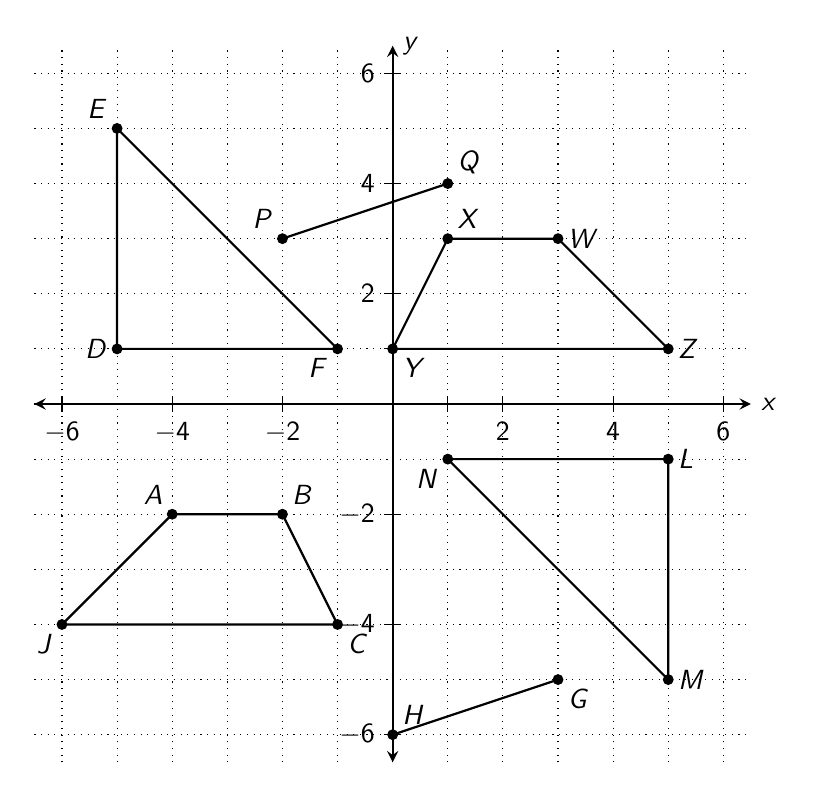
\begin{tikzpicture}[scale=0.7]
    \draw[dotted] (-6.5,-6.5) grid (6.5,6.5);
    \draw[thick, <->] (-6.5,0) -- (6.5,0) node [right] {$x$};
    \draw[thick, <->] (0,-6.5) -- (0,6.5) node [right] {$y$};
    \foreach \x in {-6,-4,-2,,2,4,6}
    \draw (\x, 0.15) -- (\x, -0.15) node [below] {$\x$};
    \foreach \y in {-6,-4,-2,,2,4,6}
    \draw (0.15,\y) -- (-0.15,\y) node [left] {$\y$};
    \coordinate (A) at (-4,-2);
    \coordinate (B) at (-2,-2);
    \coordinate (C) at (-1,-4);
    \coordinate (D) at (-5,1);
    \coordinate (E) at (-5,5);
    \coordinate (F) at (-1,1);
    \coordinate (G) at (3,-5);
    \coordinate (H) at (0,-6);
    \coordinate (J) at (-6,-4);
    \coordinate (L) at (5,-1);
    \coordinate (M) at (5,-5);
    \coordinate (N) at (1,-1);
    \coordinate (P) at (-2,3);
    \coordinate (Q) at (1,4);
    \coordinate (W) at (3,3);
    \coordinate (X) at (1,3);
    \coordinate (Y) at (0,1);
    \coordinate (Z) at (5,1);
    \draw[thick] (A) -- (B) -- (C) -- (J) -- cycle;
    \draw[thick] (D) -- (E) -- (F) -- cycle;
    \draw[thick] (P) -- (Q);
    \draw[thick] (G) -- (H);
    \draw[thick] (M) -- (N) -- (L) -- cycle;
    \draw[thick] (W) -- (X) -- (Y) -- (Z) -- cycle;
    \draw[fill=black] (A) circle [radius = 2.5pt] node [above left] {$A$};
    \draw[fill=black] (B) circle [radius = 2.5pt] node [above right] {$B$};
    \draw[fill=black] (C) circle [radius = 2.5pt] node [below right] {$C$};
    \draw[fill=black] (D) circle [radius = 2.5pt] node [left] {$D$};
    \draw[fill=black] (E) circle [radius = 2.5pt] node [above left] {$E$};
    \draw[fill=black] (F) circle [radius = 2.5pt] node [below left] {$F$};
    \draw[fill=black] (G) circle [radius = 2.5pt] node [below right] {$G$};
    \draw[fill=black] (H) circle [radius = 2.5pt] node [above right] {$H$};
    \draw[fill=black] (J) circle [radius = 2.5pt] node [below left] {$J$};
    \draw[fill=black] (L) circle [radius = 2.5pt] node [right] {$L$};
    \draw[fill=black] (M) circle [radius = 2.5pt] node [right] {$M$};
    \draw[fill=black] (N) circle [radius = 2.5pt] node [below left] {$N$};
    \draw[fill=black] (P) circle [radius = 2.5pt] node [above left] {$P$};
    \draw[fill=black] (Q) circle [radius = 2.5pt] node [above right] {$Q$};
    \draw[fill=black] (W) circle [radius = 2.5pt] node [right] {$W$};
    \draw[fill=black] (X) circle [radius = 2.5pt] node [above right] {$X$};
    \draw[fill=black] (Y) circle [radius = 2.5pt] node [below right] {$Y$};
    \draw[fill=black] (Z) circle [radius = 2.5pt] node [right] {$Z$};
\end{tikzpicture}

\newpage 

\item \mbox{} \newline 

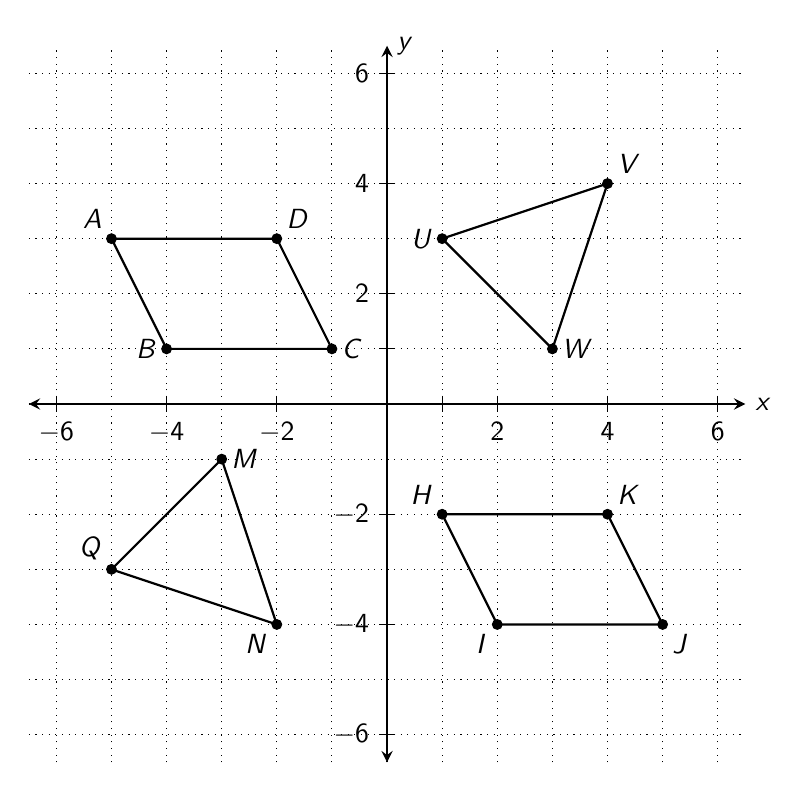
\begin{tikzpicture}[scale=0.7]
    \draw[dotted] (-6.5,-6.5) grid (6.5,6.5);
    \draw[thick, <->] (-6.5,0) -- (6.5,0) node [right] {$x$};
    \draw[thick, <->] (0,-6.5) -- (0,6.5) node [right] {$y$};
    \foreach \x in {-6,-4,-2,,2,4,6}
    \draw (\x, 0.15) -- (\x, -0.15) node [below] {$\x$};
    \foreach \y in {-6,-4,-2,,2,4,6}
    \draw (0.15,\y) -- (-0.15,\y) node [left] {$\y$};
    \coordinate (A) at (-5,3);
    \coordinate (B) at (-4,1);
    \coordinate (C) at (-1,1);
    \coordinate (D) at (-2,3);
    \coordinate (U) at (1,3);
    \coordinate (V) at (4,4);
    \coordinate (W) at (3,1);
    \coordinate (H) at (1,-2);
    \coordinate (I) at (2,-4);
    \coordinate (J) at (5,-4);
    \coordinate (K) at (4,-2);
    \coordinate (N) at (-2,-4);
    \coordinate (M) at (-3,-1);
    \coordinate (Q) at (-5,-3);
    \draw[thick] (A) -- (B) -- (C) -- (D) -- cycle;
    \draw[thick] (U) -- (V) -- (W) -- cycle;
    \draw[thick] (H) -- (I) -- (J) -- (K) -- cycle;
    \draw[thick] (Q) -- (M) -- (N) -- cycle;
    \draw[fill=black] (A) circle [radius = 2.5pt] node [above left] {$A$};
    \draw[fill=black] (B) circle [radius = 2.5pt] node [left] {$B$};
    \draw[fill=black] (C) circle [radius = 2.5pt] node [right] {$C$};
    \draw[fill=black] (D) circle [radius = 2.5pt] node [above right] {$D$};
    \draw[fill=black] (U) circle [radius = 2.5pt] node [left] {$U$};
    \draw[fill=black] (V) circle [radius = 2.5pt] node [above right] {$V$};
    \draw[fill=black] (W) circle [radius = 2.5pt] node [right] {$W$};
    \draw[fill=black] (M) circle [radius = 2.5pt] node [right] {$M$};
    \draw[fill=black] (N) circle [radius = 2.5pt] node [below left] {$N$};
    \draw[fill=black] (Q) circle [radius = 2.5pt] node [above left] {$Q$};
    \draw[fill=black] (K) circle [radius = 2.5pt] node [above right] {$K$};
    \draw[fill=black] (J) circle [radius = 2.5pt] node [below right] {$J$};
    \draw[fill=black] (I) circle [radius = 2.5pt] node [below left] {$I$};
    \draw[fill=black] (H) circle [radius = 2.5pt] node [above left] {$H$};
\end{tikzpicture}
\end{enumerate}
\end{example}

\bigskip 

\begin{example}
Given each pair of congruent triangles, find a congruence transformation that maps
\begin{multicols}{2}
\begin{enumerate}[(a)]
    \item $\triangle JQV \text{ onto } \triangle EWT$
    \item $\triangle NAV \text{ onto } \triangle BCY$
\end{enumerate}
\end{multicols}
\begin{minipage}{0.5\textwidth}
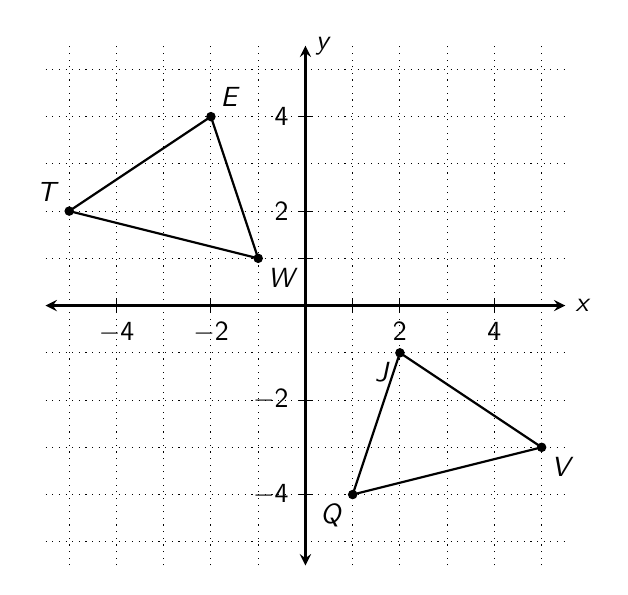
\begin{tikzpicture}[scale=0.6]
    \draw[dotted] (-5.5,-5.5) grid (5.5,5.5);
    \draw[thick, <->] (-5.5,0) -- (5.5,0) node [right] {$x$};
    \draw[thick, <->] (0,-5.5) -- (0,5.5) node [right] {$y$};
    \foreach \x in {-4,-2,,2,4}
    \draw (\x, 0.15) -- (\x, -0.15) node [below] {$\x$};
    \foreach \y in {-4,-2,,2,4}
    \draw (0.15,\y) -- (-0.15,\y) node [left] {$\y$};
    \coordinate (E) at (-2,4);
    \coordinate (W) at (-1,1);
    \coordinate (T) at (-5,2);
    \coordinate (J) at (2,-1);
    \coordinate (V) at (5,-3);
    \coordinate (Q) at (1,-4);
    \draw[thick] (E) -- (W) -- (T) -- cycle;
    \draw[thick] (J) -- (V) -- (Q) -- cycle;
    \draw[fill=black] (E) circle [radius = 2.5pt] node [above right] {$E$};
    \draw[fill=black] (W) circle [radius = 2.5pt] node [below right] {$W$};
    \draw[fill=black] (T) circle [radius = 2.5pt] node [above left] {$T$};
    \draw[fill=black] (J) circle [radius = 2.5pt] node [below left] {$J$};
    \draw[fill=black] (Q) circle [radius = 2.5pt] node [below left] {$Q$};
    \draw[fill=black] (V) circle [radius = 2.5pt] node [below right] {$V$};
\end{tikzpicture}
\end{minipage}
\begin{minipage}{0.45\textwidth}
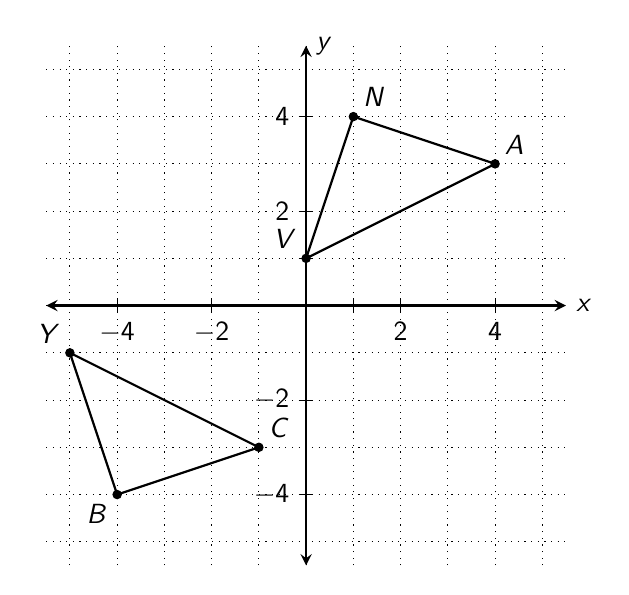
\begin{tikzpicture}[scale=0.6]
    \draw[dotted] (-5.5,-5.5) grid (5.5,5.5);
    \draw[thick, <->] (-5.5,0) -- (5.5,0) node [right] {$x$};
    \draw[thick, <->] (0,-5.5) -- (0,5.5) node [right] {$y$};
    \foreach \x in {-4,-2,,2,4}
    \draw (\x, 0.15) -- (\x, -0.15) node [below] {$\x$};
    \foreach \y in {-4,-2,,2,4}
    \draw (0.15,\y) -- (-0.15,\y) node [left] {$\y$};
    \coordinate (N) at (1,4);
    \coordinate (A) at (4,3);
    \coordinate (V) at (0,1);
    \coordinate (B) at (-4,-4);
    \coordinate (C) at (-1,-3);
    \coordinate (Y) at (-5,-1);
    \draw[thick] (N) -- (A) -- (V) -- cycle;
    \draw[thick] (B) -- (C) -- (Y) -- cycle;
    \draw[fill=black] (N) circle [radius = 2.5pt] node [above right] {$N$};
    \draw[fill=black] (A) circle [radius = 2.5pt] node [above right] {$A$};
    \draw[fill=black] (V) circle [radius = 2.5pt] node [above left] {$V$};
    \draw[fill=black] (B) circle [radius = 2.5pt] node [below left] {$B$};
    \draw[fill=black] (C) circle [radius = 2.5pt] node [above right] {$C$};
    \draw[fill=black] (Y) circle [radius = 2.5pt] node [above left] {$Y$};
\end{tikzpicture}
\end{minipage}
\end{example}

\end{document}
